\documentclass[10pt,article]{article}
\newcommand{\myMargin}{0.2in}
\usepackage[a4paper, margin=\myMargin]{geometry}
\usepackage{graphicx}
\usepackage{booktabs}
\usepackage{url}
\usepackage{enumitem}
\usepackage{palatino}
\usepackage{tabularx}
\usepackage{multicol}
\usepackage{xcolor}
\usepackage{enumitem}
\usepackage[hidelinks]{hyperref}
\fontfamily{SansSerif}
\usepackage{multirow}
% \usepackage{fontspec}
\usepackage{fontawesome}
% \usepackage[T1]{fontenc}

\selectfont

\usepackage[T1]{fontenc}
\usepackage
%[ansinew]
[utf8]
{inputenc}

\usepackage{color}
% \definecolor{myblue}{gray}{0.82}
\definecolor{myblue}{HTML}{96bfeb}
\definecolor{myred}{HTML}{961212}
\definecolor{nptel}{HTML}{c71254}
\textheight=10.75in
\raggedbottom

\setlength{\tabcolsep}{0in}
\newcommand{\isep}{-2 pt}
\newcommand{\lsep}{-0.5cm}
\newcommand{\psep}{-0.6cm}
\renewcommand{\labelitemii}{$\circ$}

\pagestyle{empty}
%-----------------------------------------------------------
%Custom commands
\newcommand{\resitem}[1]{\item #1 \vspace{-2pt}}
% \newcommand{\resheading}[1]{{\small \colorbox{myblue} { \begin{minipage}{0.99\textwidth}\centering{\textbf{#1 \vphantom{p\^{E}}}}\end{minipage}}}}
% \newcommand{\ressubheading}[3]{
% \begin{tabular*}{6.62in}{l @{\extracolsep{\fill}} r}
% 	\textsc{{\textbf{#1}}} & \rightline\textsc{\textit{[#2]}} \\
% \end{tabular*}\vspace{-8pt}}

\newcommand{\resheading}[1]{{\small \colorbox{myblue} { \begin{minipage}{\dimexpr\linewidth-2\fboxsep}\centering{\textbf{#1 \vphantom{p\^{E}}}}\end{minipage}}}}

\newcommand{\ressubheading}[3]{
\begin{tabular*}{\linewidth}{@{}l @{\extracolsep{\fill}} r@{}}
    \textsc{\textbf{#1}} & \textsc{\textit{[#2]}} \\
\end{tabular*}\vspace{-8pt}}

% New command for font size
\newcommand{\myfont}[2]{\fontsize{#1}{#1}\selectfont #2}

% New command for Subheading font size
\newcommand{\subheadingfont}[1]{\myfont{11pt}{#1}}

% New command for Project Topic name 
\newcommand{\projecttopic}[1]{\myfont{11pt}{\textbf{#1}}}

% New command for Project Description
\definecolor{projDescColor}{HTML}{1923A8}
\newcommand{\projectdesc}[1]{\myfont{10pt}{\textcolor{projDescColor}{\textit{#1}}}}

% New command for Link
\newcommand{\mylink}[1]{\href{#1}{
\includegraphics[scale=0.03]{download.png}}}

% New command for Calendar
\newcommand{\mycal}[1]{
\includegraphics[scale=0.02]{calendar.png} \myfont{10}{#1}}

%%%%%%%%%%%%%%%%%%%%%%%%%%%%%%%%%%%%%%%%%%%%%%%%%%%%%%%%%%%%%%%%%%%%%%%%%%%%%%%%%%%%%%%%%%%%%%%%%%%%%%%%%%

\begin{document}
\begin{table}
    \begin{minipage}{0\linewidth}
        \centering
        
\includegraphics[height =1in]{Logo.png}
    \end{minipage}
    \begin{minipage}{0.9\linewidth}
        %\centering
        \setlength{\tabcolsep}{70pt}
        \def\arraystretch{1.1}
        \begin{tabular}{l l r}
            \textbf{\Large{Snehadeep Gayen $\vert$ CS21B078}} &
            \multirow{3}{*}{     {\href{https://github.com/Snehadeep-Gayen}{
\includegraphics[scale=0.05]{github.png}} \ 
 \href{https://www.linkedin.com/in/snehadeep-gayen/}{
\includegraphics[scale=0.05]{linkedin.png}} \ \href{https://codeforces.com/profile/Snehadeep}{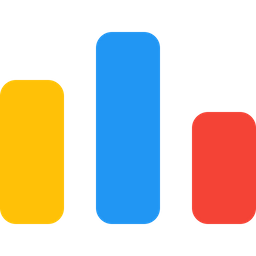
\includegraphics[scale=0.06]{cf.png} \ } 
            }}
            % &  {\href{https://github.com/Snehadeep-Gayen}{
\includegraphics[scale=0.03]{github.png}} \  Snehadeep-Gayen} 
            \\
            \textbf{B. Tech Computer Science and Engineering} 
            \\
            {Indian Institute of Technology, Madras} 
            % &    {\href{https://codeforces.com/profile/Snehadeep}{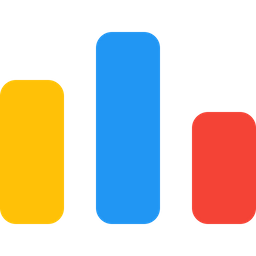
\includegraphics[scale=0.04]{cf.png}} \ Snehadeep} 
            \\
        \end{tabular}
    \end{minipage}\hfill
\end{table}

%%%%%%%%%%%%%%%%%%%%%%%%%%%%%%%%%%%%%%%%%%%%%%%%%%%%%%%%%%%%%%%%%%%%%%%%%%%%%%%%%%%%%%%%%%%%%%%%%%%%%%%%%%

\setlength{\tabcolsep}{20pt}
\begin{table}
\centering
\noindent
\resheading{\subheadingfont{EDUCATION}}\\ 
\vspace{5pt}
\begin{tabular}{lllll}
\toprule
\toprule
\textbf{Course}  & \textbf{CGPA/\%}  & \textbf{Institution} & \textbf{Year} \\ 
\toprule
 B. Tech CSE  & \fontsize{11pt}{12pt} \selectfont \textbf{9.90} & Indian Institute of Technology, Madras & 2021-Present  \\ 
HSC 12$^{th}$ & 98.17  & Pace Junior Science College Andheri, Mumbai & 2019-21  \\ 
ICSE 10$^{th}$ & 98.8 &  Lilavatibai Podar High School, Mumbai & 2019\\ 
\bottomrule
\bottomrule \\[-0.9cm]
\end{tabular}
\end{table}

%%%%%%%%%%%%%%%%%%%%%%%%%%%%%%%%%%%%%%%%%%%%%%%%%%%%%%%%%%%%%%%%%%%%%%%%%%%%%%%%%%%%%%%%%%%%%%%%%%%%%%%%%%

\begin{multicols*}{2}
\noindent
\resheading{\subheadingfont{PROJECTS} }\\[0.1cm]

\noindent
\projecttopic{WiFi Tomography} \textit{\myfont{9pt}{(Ongoing)}} \hfill \textcolor{projDescColor}{\textit{Python}}  \\
\projectdesc{Project Under Prof. Ayon Chakraborty} \hfill \mycal{May'23 - Present} 
\begin{itemize}[nolistsep, leftmargin=\myMargin]
    \item WiFi tomography is a low-cost and easily implementable method to image the environment using WiFi signals.
    \item Working on computational optimisation of Tomographic Reconstruction to make it suitable for outdoor
        and indoor drone application 
\end{itemize} 

\noindent
\

% \noindent
% \projecttopic{Hack CPU} \mylink{https://github.com/Snehadeep-Gayen/Computer-Organisation-and-Architecture-Lab} \hfill \textit{Verilog} \\
% \projectdesc{CS2610 Course Project - Prof. C Chandra Sekhar} \hfill \mycal{Jan'23 - May '23}
% \begin{itemize}[noitemsep]
%     \item Implemented a CPU with register file and ALU with instructions to perform Arithmetic and Logical operations on both 8-bit integers and  12-bit floating-point numbers
% \end{itemize}

% \noindent
% \projecttopic{Simple CPU} \mylink{https://github.com/Snehadeep-Gayen/Simple_CPU_Design} \hfill \textit{Verilog} \\
% \projectdesc{CS2310 Course Project - Prof. Ayon Chakraborty} \hfill \mycal{Jul'22 - Nov'22}
% \begin{itemize}[noitemsep]
%     \item Built a combinational 8-bit CPU (from gate level) using HDL (Verilog) as a part of course CS2310
% \end{itemize}

\noindent
\projecttopic{CPU Design} \mylink{https://github.com/Snehadeep-Gayen/Computer-Organisation-and-Architecture-Lab} 
\mylink{https://github.com/Snehadeep-Gayen/Simple_CPU_Design} 
\hfill    \textcolor{projDescColor}{\textit{Verilog}}  \\
\projectdesc{CS2610 Course Project - Prof. C. Chandra Sekhar} \hfill \mycal{Jan-May '23} \\
\projectdesc{CS2310 Course Project - Prof. Ayon Chakraborty} \hfill \mycal{Jul-Nov '22}
\noindent
\begin{itemize}[nolistsep, leftmargin=\myMargin]
    \item Implemented a CPU with register file and ALU with instructions to perform Arithmetic 
    and Logical operations on both 8-bit integers and  12-bit floating-point numbers
    \item Built a combinational 8-bit CPU from gate level
\end{itemize}

\noindent
\


\noindent
\projecttopic{Reading Project and Presentation} \mylink{https://docs.google.com/presentation/d/11JGNKZnVHHQ-aGJLIgkdXcnK5qy_xisO/edit?usp=sharing&ouid=111499804735475673896&rtpof=true&sd=true} \\
\projectdesc{CS6122 Course Project - Prof. B. V. R. Rao} \hfill \mycal{Jan-May '23} 
\begin{itemize}[noitemsep, nolistsep, leftmargin=\myMargin]
    \item Presented the paper on \href{https://doi.org/10.1007/s00453-012-9643-5}{\textit{``Smoothed Analysis of Partitioning Algorithms for Euclidean Functionals"} 
    by \textit{Bläser, M., Manthey, B. \& Rao, B.V.R.}} and discussed its applications to problems
\end{itemize}

\noindent
\


\noindent
\projecttopic{Closeness Centrality Algorithm} \mylink{https://github.com/Snehadeep-Gayen/CENDY-Incremental-CC}
 \hfill \textcolor{projDescColor}{\textit{C++}} \\
\projectdesc{Project under Prof. Manikandan Narayanan} \hfill \mycal{May-Jun '23}
\begin{itemize}[nolistsep, leftmargin=\myMargin]
    \item Implemented the CENDY algorithm based on this paper \ \mylink{https://ieeexplore.ieee.org/stamp/stamp.jsp?tp=&arnumber=6729571&isnumber=6729471}
    \item This on-line algorithm updates Average Path Length and Closeness Centrality of all nodes
    in a Dynamic Graph
 \end{itemize}


% \begin{itemize}
% \setlength\itemsep{-0.5em}


% \item \textbf{WiFi Tomography* \big\vert \   Prof. Ayon Chakraborty} \hfill { \textit{Python}} \\
%  \\[-1cm]
% \begin{itemize}[noitemsep]
%     \item Working on computational optimisation of Tomographic Imaging (using WiFi) for outdoor
%     and indoor drone application 
%  \end{itemize}
 
% \item \textbf{Hack CPU \big\vert \   Prof. C Chandra Sekhar} \  \href{https://github.com/Snehadeep-Gayen/Computer-Organisation-and-Architecture-Lab}{
\includegraphics[scale=0.03]{download.png}} \hfill {\textit{Verilog} } 
% \begin{itemize}[noitemsep,nolistsep]
%     \item Implemented a CPU with register file and ALU with instructions to perform Arithmetic and Logical operations on both 8-bit integers and  12-bit floating-point numbers as a part of course CS2610
%  \end{itemize}
% \vspace{5pt}
 
% \item \textbf{Simple CPU \big\vert \   Prof. Ayon Chakraborty} \ \href{https://github.com/Snehadeep-Gayen/Simple_CPU_Design}{
\includegraphics[scale=0.03]{download.png}} \hfill {\textit{Verilog} } 
% \begin{itemize}[noitemsep,nolistsep]
%     \item Built a combinational 8-bit CPU (from gate level) using HDL (Verilog) as a part of course CS2310
%  \end{itemize}
%  \vspace{5pt}
 
% \end{itemize}

%%%%%%%%%%%%%%%%%%%%%%%%%%%%%%%%%%%%%%%%%%%%%%%%%%%%%%%%%%%%%%%%%%%%%%%%%%%%%%%%%%%%%%%%%%%%%%%%%%%%%%%%%%
\noindent
\resheading{\subheadingfont{EXPERIENCE}} \\
% \begin{itemize}
% \setlength\itemsep{-0.1em}
% \item \textbf{Member, Team Avishkar Hyperloop 6.0 \ \big\vert \   C\textcolor{red}{FI} IITM}   
% % \  \parbox{\linewidth}{\hfill \textit{Oct '22 - Present}}
%  \\[-0.5cm]
% \begin{itemize}[noitemsep,nolistsep]
%     \item Participated in the prestigious \textbf{European\\ Hyperloop Week} representing IITM \& India
%     \item Part of the design and implementation team of the Main Control Unit and Nagivation Unit of our Pod
%     \item Used RTOS and comm. protocols like MQTT, CAN, etc to collect and store data from over 20 sensors at \textbf{low latency}, \textbf{handling faults} appropriately.
%  \end{itemize}
% \item \textbf{Tutor \& Contributor \big\vert \   NPTEL }\hfill \textit{March '23 - Present} 
% \begin{itemize}[noitemsep,nolistsep]
%     \item Created \textbf{YouTube tutorials} under NPTEL for \\ previous year GATE CS questions especially \\ for the less privelleged applicants
%  \end{itemize}

% \end{itemize}

%%%%%%%%%%%%%%%%%%%%%%%%%%%%%%%%%%%%%%%%%%%%%%%%%%%%%%%%%%%%%%%%%%%%%%%%%%%%%%%%%%%%%%%%%%%%%%%%%%%%%%%%%%

\noindent
\projecttopic{Team Avishkar Hyperloop, C\textcolor{red}{FI}} \hfill \mycal{Oct '22 - Present} 
\begin{itemize}[noitemsep, nolistsep, leftmargin=\myMargin]
    \item Part of Design \& Code Development Team of the Main Control Unit and Navigation Unit of our Pod. 
    \item Used RTOS and threading to collect and store data from over 20 sensors at \textbf{low latency}, \textbf{handling faults} appropriately.
    \item Used communication protocols like MQTT, CAN, etc to collect data and send data to the base station/on-Pod Storage.
    \item Participated in prestigious \textbf{European Hyperloop Week - Scotland 2023}, 
    among over 25 teams globally to represent the country.
\end{itemize}
\noindent
\ 
\projecttopic{Tutor \& Contributor, \textcolor{nptel}{NPTEL}} \hfill \mycal{March '23 - Present} 
\begin{itemize}[noitemsep, nolistsep, leftmargin=\myMargin]
    \item Created \textbf{YouTube tutorials} under NPTEL for previous year GATE CS questions especially for the less privelleged applicants
\end{itemize}


%%%%%%%%%%%%%%%%%%%%%%%%%%%%%%%%%%%%%%%%%%%%%%%%%%%%%%%%%%%%%%%%%%%%%%%%%%%%%%%%%%%%%%%%%%%%%%%%%%%%%%%%%%
  

\columnbreak


%%%%%%%%%%%%%%%%%%%%%%%%%%%%%%%%%%%%%%%%%%%%%%%%%%%%%%%%%%%%%%%%%%%%%%%%%%%%%%%%%%%%%%%%%%%%%%%%%%%%%%%%%%

\noindent
\resheading{\subheadingfont{SCHOLASTIC ACHIEVEMENTS}}
\begin{itemize}[leftmargin=\myMargin]
\setlength \itemsep{-0.1em}
\item Secured \textbf{AIR 5} in JEE Mains out of 1 million students  %\hfill {[20XX]}%
\item Secured \textbf{AIR 161} in JEE Advanced \hfill
\item Secured \textbf{AIR 10} in Indian Statistical Institute Exam
\item Secured \textbf{AIR 21} in INChO and attended IChO Camp
\item Awarded KVPY Fellowship (2021) with \textbf{AIR 338}
\item Winner of Mimamsa '22 at IISER Pune \\ 4$^{th}$ place in Chemenigma '22 at IISC Bangalore \& \\ Won Silver Medal in Homi Bhabha Science Competition \\ (conducted in Maharashtra)
\end{itemize} 

%%%%%%%%%%%%%%%%%%%%%%%%%%%%%%%%%%%%%%%%%%%%%%%%%%%%%%%%%%%%%%%%%%%%%%%%%%%%%%%%%%%%%%%%%%%%%%%%%%%%%%%%%%
 

%%%%%%%%%%%%%%%%%%%%%%%%%%%%%%%%%%%%%%%%%%%%%%%%%%%%%%%%%%%%%%%%%%%%%%%%%%%%%%%%%%%%%%%%%%%%%%%%%%%%%%%%%%

\noindent
\resheading{\subheadingfont{CODING ACHIEVEMENTS}}
 \begin{itemize}[ leftmargin=\myMargin]
    \setlength \itemsep{-0.1em}
  \item Maximum Rating 1678 \textcolor{blue}{(Expert)} on Codeforces
%   \item Maximum Rating 1653 \textcolor{blue}{(3 
\includegraphics[scale=0.03]{bluestar.png})} on CodeChef
  \item \textbf{ICPC 2022} - \textbf{AIR 151} and \textbf{Institute Rank 7} in Kanpur-Mathura Qualifier Round
\item \textbf{AIR 3} in Shaastra CP Potpourri (Mixed-bag coding contest) \\ \small {\textit{[Shaastra is Asia's largest student-run Techfest]}} 
    \item \normalsize{ \textbf{Global Rank 9} in CodeChef Starters 96} 
    \item \normalsize{ \textbf{Global Rank 231} in Codeforces Round 881} 
    \item \normalsize{ \textbf{Global Rank 373} in Google Farewell Round} 
    \item  \normalsize {1st place in Inter-School Java Competition in Mumbai}
  \end{itemize}

%%%%%%%%%%%%%%%%%%%%%%%%%%%%%%%%%%%%%%%%%%%%%%%%%%%%%%%%%%%%%%%%%%%%%%%%%%%%%%%%%%%%%%%%%%%%%%%%%%%%%%%%%%



 
\noindent
\resheading{\subheadingfont{SOFTWARE SKILLS}}
 \begin{itemize}[leftmargin=\myMargin]
    \setlength \itemsep{-0.1em}
  \item \textbf{Languages}: C++, C, HDL (Verilog), Python, Java, HTML, CSS, x86, RISC and 8085 ASM, R
  \item \textbf{Tools}: TI CCS, Git, \textbf{\LaTeX}, AutoCAD, GDB
\item \textbf{Libraries}: TI RTOS, NumPy, PyLops, Matplotlib
  \end{itemize}
  
%%%%%%%%%%%%%%%%%%%%%%%%%%%%%%%%%%%%%%%%%%%%%%%%%%%%%%%%%%%%%%%%%%%%%%%%%%%%%%%%%%%%%%%%%%%%%%%%%%%%%%%%%%

\noindent
\resheading{\subheadingfont{EXTRACURRICULAR ACTIVITIES}}
\begin{itemize}[leftmargin=\myMargin]
    \setlength \itemsep{-0.1em}
\item \textbf{Sports:} Taekwondo Red Dan II Belt, Awarded Best \\ Athlete U14 at School, NSO Athlete at IITM
\item Mentored freshmen, personally and academically, \\ under \textbf{Saathi, IIT Madras}
\item Avid book reader and Tabla player
\end{itemize}

\noindent
\resheading{\subheadingfont{COURSES \& LABS}}
 % \textbf{Econometrics \big\vert \   Statistics \big\vert \   Mathematical Methods \big\vert \   Microeconomics \big\vert \   Macroeconomics}\hfill {[ISI-D]}\\[-0.1cm]\\
\begin{multicols}{2} 


%%%%%%%%%%%%%%%%%%%%%%%%%%%%%%%%%%%%%%%%%%%%%%%%%%%%%%%%%%%%%%%%%%%%%%%%%%%%%%%%%%%%%%%%%%%%%%%%%%%%%%%%%%

\begin{itemize}[noitemsep, nolistsep, leftmargin=\myMargin]
  % \item {\small Problem Solving using Computers} 
  \item { Basic Electrical Engg} 
  \item { Computer Systems Design} 
  \item {Programming and Data Structures}
  \item { Computer Organisation and Architecture} 
  \item { Design \& Analysis of Algorithms} 
  \item { Theory of Computation} 
  \item { Probabilistic, Smoothed Analysis of Algorithms} 
  \item { Object Oriented Programming} 
  \item { Discrete Maths} 
  \item { Basic Grpah Theory} 
  \item { Probability, Statistics\& Stochastic Processes} 
  \item { Series and Matrices} 
  \item { Multivariable Calculus} 
  \item { Ordinary Differential Eqns}  
  \item { Principles of Economics} 
  \item { Intro to Game Theory}   
  \item { Compiler Design *} 
  \item { Operating System *}
\end{itemize}
\hfill  {* ~ Ongoing}

\end{multicols}

%%%%%%%%%%%%%%%%%%%%%%%%%%%%%%%%%%%%%%%%%%%%%%%%%%%%%%%%%%%%%%%%%%%%%%%%%%%%%%%%%%%%%%%%%%%%%%%%%%%%%%%%%%

\end{multicols*}
\end{document}